\chapter{Goal Diagram}
I goal rappresentano degli \textit{statement} prescrittivi delle 
proprietà che il sistema deve avere attraverso la cooperazione 
di più agenti. Tali \textit{statement} sono realizzati attraverso la 
terminologia e il dominio nella quale il sistema opera e 
sono a vari livelli di granularità.

per capire se un ci troviamo di fronte ad un goal dobbiamo capire 
se questa proprietà può essere negoziata, indebolita o rafforzata.
Altrimenti ci troviamo di fronte ad una proprietà 
di dominio.


\section{Rappresentazione dei Goal}
All'interno del goal diagram i goal vengono rappresentati con 
un parallelogramma che può o meno avere il bordo in grassetto.
\begin{figure}[H]
    \centering
    \begin{tikzpicture}
        \node[draw=black, fill=blue!20, trapezium, trapezium left angle=70, trapezium right angle=110] (goal) {DoorClosedWhileMoving};
        \node[draw=black, fill=blue!20, trapezium, trapezium left angle=70, trapezium right angle=110, ultra thick, right=of goal] (goal2) {BlockSpeedLimited};
    \end{tikzpicture}
    \caption{Rappresentazione di un goal}
\end{figure}
Possono avere delle annotazioni per specificare ulteriori attributi 
di questo goal, e possono avere delle precise definizioni a 
seconda del progetto software.

\section{Raffinamento dei goal}
Il raffinamento permette di suddividere un goal in sotto-goal
per poterlo realizzare. Questo raffinamento può essere di due tipi:
\begin{itemize}
    \item \texttt{AND}-refinement.
    \item \texttt{OR}-refinement.
\end{itemize}
\section{\texttt{AND}-refinement}
Nell'\texttt{AND}-refinement il goal viene suddiviso in sotto-goal 
che devono essere soddisfatti tutti per poter soddisfare il goal 
principale.
    \begin{figure}[H]
        \centering
        \begin{tikzpicture}
            % Nodo superiore
            \node[draw=black, fill=blue!20, trapezium, trapezium left angle=70, trapezium right angle=110] (goal1) {TrainStoppedAtStation};

            % Nodo centrale con "AND-refinement"
            \node[below=1cm of goal1] (and) [circle, draw, fill=yellow] {};
            \node[right=0.5cm of and] (and_text) {\textcolor{red}{\textit{AND-refinement}}};

            % Nodi inferiori
            \node[draw=black, fill=blue!20, trapezium, trapezium left angle=70, trapezium right angle=110, thick, below left=1cm and 3.5cm of and] (goal2) {speedAchievedIsZero};
            \node[draw=black, fill=blue!20, trapezium, trapezium left angle=70, trapezium right angle=110, thick, below right=1cm and 3.5cm of and] (goal3) {radarDetectedStation};

            % Frecce di collegamento
            \draw[->] (and) -- (goal1);
            \draw[->] (goal2) -- (and);
            \draw[->] (goal3) -- (and);
        \end{tikzpicture}
        \caption{Rappresentazione di una raffinamento di tipo \texttt{AND}}
    \end{figure}
    Il raffinamento di tipo \texttt{AND} deve essere \textbf{completo}, ciò significa 
    che il raggiungimento degli obiettivi in \texttt{AND} è una condizione sufficiente 
    per il raggiungimento del goal di più alto livello.
    \[
    \{ G_1, G_2, \ldots, G_n \} \models G
    \]

\subsection{Proprietà di dominio}
    \begin{figure}[H]
        \centering
        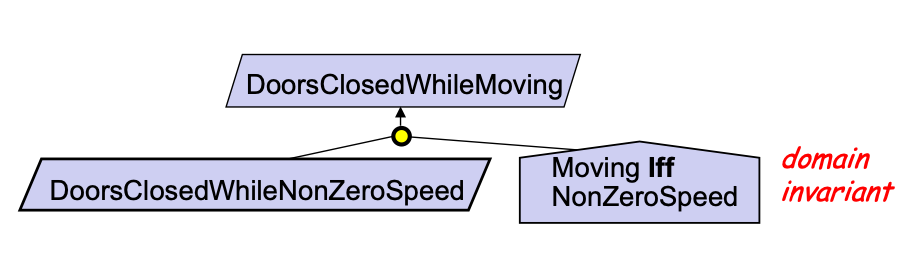
\includegraphics[width=0.7\textwidth]{img/domain.png}
        \caption{Rappresentazione di una proprietà di dominio}
    \end{figure}
    \begin{itemize}
        \item \textbf{Invariante di dominio}: proprietà di dominio che non varia.
        \item \textbf{Ipotesi di dominio}: proprietà di dominio che assume una condizione.
    \end{itemize}
\subsection{Altre proprietà}
\begin{itemize}
    \item \textbf{Consistenza}: non ci sono contraddizioni tra il goal e i suoi raffinamenti.
    Quindi non accade che:
    \[
    \{ G_1, G_2, \ldots, G_n, Dom \} \models \texttt{false}
    \]
    \item \textbf{Minimalità}: se viene tolto anche solo un sotto-goal il goal principale
    non può essere raggiunto.
    \[
    \{ G_1, G_2, \ldots, G_{j-1}, G_{j+1}, \ldots, G_n \} \not\models G
    \]
\end{itemize}
\subsection{Alberi di raffinamento}
\begin{tcolorbox}[colback=violet!5!white,colframe=violet!75!black, title=Requisito]
    Un requisito è un goal che non può essere raffinato ulteriormente.
\end{tcolorbox}
Quando ho un goal che è responsabilità di un solo agente, allora posso 
fermare il raffinamento.
\subsection{Potenziali conflitti}
La presenza di contraddizioni potrebbe far emergere nuovi requisiti, rappresentando quindi 
delle temporanee lacune nella modellazione, non essendo quindi un pattern da evitare. È piuttosto 
importante documentare questi conflitti per poterli risolvere in seguito, attraverso un artefatto.
\begin{figure}[H]
    \centering
    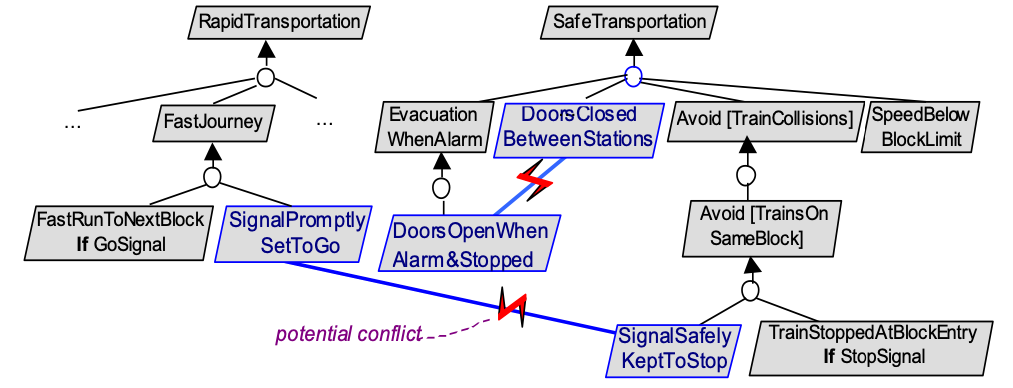
\includegraphics[width=0.9\textwidth]{img/conflitto.png}
    \caption{Rappresentazione di un conflitto}
\end{figure}
\section{\texttt{OR}-decomposition}
Nella \textbf{\texttt{OR}-refinement} il goal viene suddiviso in sotto-goal 
che devono essere soddisfatti almeno uno per poter soddisfare il goal 
principale.
\begin{figure}[H]
        \centering
        \begin{tikzpicture}
            % Nodo superiore
            \node[draw=black, fill=blue!20, trapezium, trapezium left angle=70,
            trapezium right angle=110] (goal1) {Avoid [TrainCollision]};

            % Nodo centrale con "OR-refinement"
            \node[below right=1cm of goal1] (or1) [circle, draw, fill=yellow] {};
            \node[below left=1cm of goal1] (or2) [circle, draw, fill=yellow] {};
            \node[right=0.5cm of or1] (or_text) {\textcolor{red}{\textit{OR-refinement}}};

            % Nodi inferiori
            \node[draw=black, fill=blue!20, trapezium, trapezium left angle=70,
            trapezium right angle=110, thick, below left=1cm and 3.2cm of or1] (goal2)
            {Avoid [TrainOnSameBlock]};
            \node[draw=black, fill=blue!20, trapezium, trapezium left angle=70,
            trapezium right angle=110, thick, below right=1cm and 3.2cm of or2] (goal3)
            {Maintain [SafeDistance]};

            % Frecce di collegamento
            \draw[->] (or1) -- (goal1);
            \draw[->] (or2) -- (goal1);
            \draw[->] (goal2) -- (or2);
            \draw[->] (goal3) -- (or1);

        \end{tikzpicture}
        \caption{Rappresentazione di una raffinamento di tipo \texttt{OR}}
    \end{figure}
\subsection{Assegnamento di responsabilità alternativo}
Nel caso in cui un goal possa essere raggiunto da più agenti diversi, in cui 
ognuno di essi può raggiungere il goal in modo indipendente, allora si può
utilizzare un raffinamento di tipo \texttt{OR}.
\begin{figure}[H]
    \centering
    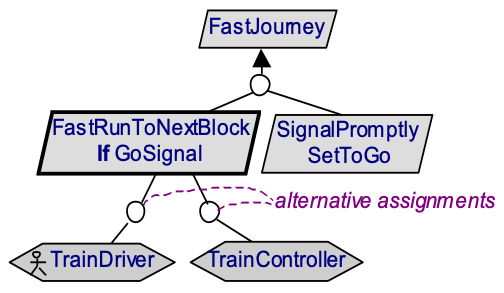
\includegraphics[width=0.6\textwidth]{img/assignmnets.png}
    \caption{Rappresentazione di un assegnamento di responsabilità alternativo}
\end{figure}
È opportuno in fase di modellazione segnalare queste alternative che verranno discusse in futuro 
sulla base di costi, benefici e rischi.
\section{Annotazioni}
Possiamo aggiungere annotazioni e commenti per specificare ulteriori dettagli liberamente 
in modo da enfatizzare o cristallizzare il significato.
\begin{figure}[H]
    \centering
    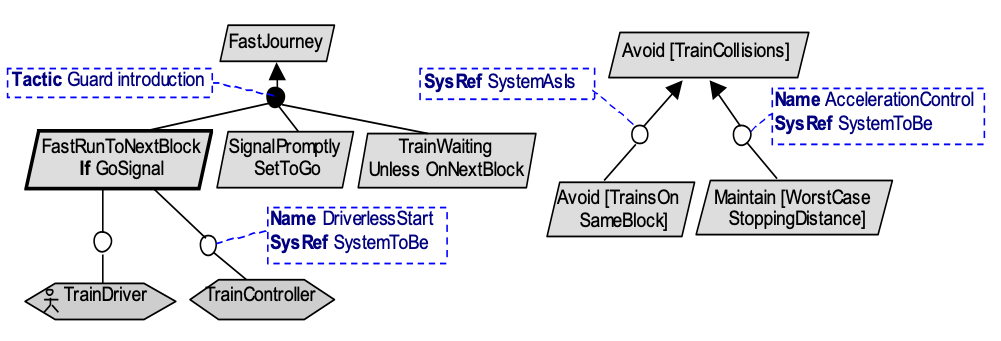
\includegraphics[width=0.9\textwidth]{img/annotazionigoal.png}
    \caption{Rappresentazione di un'annotazione}
\end{figure}
\section{Euristiche per l'individualizzazione dei goal}
\begin{itemize}
    \item Elicitazione dei goal preliminare.
    \begin{itemize}
        \item Analizzare gli obiettivi correnti del sistema \textit{as-is}.
        \item Cercare keyword all'interno del materiale elicitato.
        \item Cercare all'interno delle tassonomie di goal.
    \end{itemize}
    \item Identificare i goal lungo i branch di raffinamento.
    \begin{itemize}
        \item Farsi le domande ``Perché?'' (\textit{astrazione}), ``Come?'' (\textit{raffinamento}).
        \item Utilizzare gli scenari.
        \item Dividere le responsabilità tra gli agenti.
        \item Identificare i goal da i pro e contro.
        \item Dagli \textit{Achive goal} posso identificare i \textit{Maintain goal}.
    \end{itemize}
    \item Non confondere i goal con le operazioni.
    \item Non confondere \texttt{AND}-refinement con \texttt{OR}-refinement.
    \item Evitare ambiguità.
\end{itemize}

\chapter{Analisi dei rischi}
\begin{tcolorbox}[colback=red!5!white,colframe=red!75!black, title=Rischio]
    Un rischio è una probabilità che un goal non venga raggiunto.
\end{tcolorbox}
La funzionalità del sistema software viene a mancare, facendo si che il sistema
raggiunga dei risultati parziali. I rischi vanno modellati già nella fase di modellazione 
dei goal, in modo da individuare i goal che possono essere compromessi e come mitigare
questi rischi.

Già nella fase di modellazione dei requisiti abbiamo affrontato la risk analysis,
identificando le fasi relative ai rischi.
\begin{figure}[H]
    \centering
    \begin{tikzpicture}
        % Styles
        \tikzstyle{process} = [rectangle, rounded corners, minimum width=3cm, minimum height=1cm, text centered, draw=black, fill=blue!20, text width=2.5cm]
      
        % Nodes
        \node (start) [circle, fill, inner sep=2pt] {};
        \node (identify) [process, right=0.5cm of start]
        {Identificare \\ i rischi};
        \node (detect) [process, right=0.5cm of identify]
        {Valutazione \\ dei rischi};
        \node (evaluate) [process, right=0.5cm of detect]
        {Controllo dei \\ rischi};
      
        % Arrows
        \draw[->] (start) -- (identify);
        \draw[->] (identify) -- (detect);
        \draw[->] (detect) -- (evaluate);
        \draw[->]  (evaluate.south) -- ++(0,-0.5) -| (start.south);
    \end{tikzpicture}
\end{figure}
La mancata individuazione dei rischi è una delle principali cause di fallimento
dei progetti software. 

I rischi possono essere rappresentati attraverso un parallelogramma, inclinato
nella direzione opposta rispetto ai goal.
\begin{figure}[H]
    \centering
    \begin{tikzpicture}
        \node[draw=black, fill=red!20, trapezium, trapezium right angle=70, trapezium left angle=110] (goal) {rischio};
    \end{tikzpicture}
    \caption{Rappresentazione di un rischio}
\end{figure}

\section{Goal ostruiti dai rischi}
Quando modelliamo i goal rischiamo di modellare solamente il funzionamento 
corretto del sistema, senza considerare i rischi che possono compromettere
il raggiungimento di questi goal. 

Un \textbf{ostacolo} insieme ad una proprietà di dominio implica che il goal
non può essere raggiunto.
\[ 
\{ G, Dom \} \models \neg G
\] 

L'insieme ideale di ostacoli di $G$ dovrebbe essere la negazione di tutti 
i goal che permettono di raggiungere $G$.

Anche gli ostacoli, come i goal possono essere mappati in una tassonomia per 
poter identificare i rischi in modo più semplice.

\section{Modellazione degli ostacoli}
\begin{figure} [H]
    \centering
    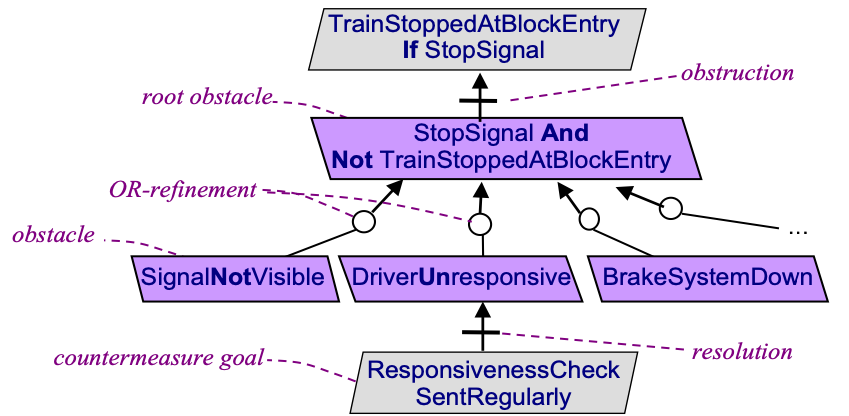
\includegraphics[width=0.9\textwidth]{img/ostruzione.png}
    \caption{Rappresentazione di un ostacolo}
\end{figure}
La modellazione è simile a quella dei goal, dove per rappresentare un ostacolo 
che potrebbe compromettere il raggiungimento di un goal, si utilizza un \textit{link di ostruzione}.
Anche qui possiamo usare la \texttt{AND}-decomposition e la \texttt{OR}-decomposition per
raffinare gli ostacoli. 

Per rappresentare una possibile soluzione ad un ostacolo si può
usare un \textit{link di risoluzione} che collega un goal ad un ostacolo.

\subsection{Raffinamento dei rischi}
La struttura dei goal è molto simile alla struttura dei rischi, quindi, molto spesso, 
si può raffinare un rischio in modo simile a come si raffina un goal.

Anche per gli ostacoli possiamo identificare delle annotazioni per specificare ulteriori dettagli.

\section{Analisi degli ostacoli per migliorare la robustezza del sistema}
I nostri obiettivi principali sono:
\begin{itemize}
    \item Identificare quanti più ostacoli possibili.
    \item Comprendere la probabilità di occorrenza di questi ostacoli.
    \item Comprendere l'impatto di questi ostacoli.
\end{itemize}
\begin{figure}[H]
    \centering
    \begin{tikzpicture}[node distance=1cm and 1cm, auto,
        mynode/.style={ellipse, draw, fill=red!30, minimum width=5em, minimum height=3em, text centered, font=\footnotesize},
        myarrow/.style={->, >=latex', thick},
        scale=0.8, every node/.style={scale=0.8}]

        % Nodes
        \node[mynode] (a) {Obstacle Identification};
        \node[mynode, right=of a] (b) {Obstacle Assessment};
        \node[mynode, right=of b] (c) {Obstacle Resolution};
        \node[mynode, above=0.75cm of b] (d) {Goal Model Elaboration};

        % Arrows
        \draw[myarrow] (a) -- (b);
        \draw[myarrow] (b) -- (c);
        \draw[myarrow] (c.north) -- (d.east);
        \draw[myarrow] (d.west) -- (a.north);

        % Self-loops with better position and style
        \path[myarrow] (a) edge [loop left] node[left] {} (a);
        \path[myarrow] (d) edge [loop above] node[above] {} (d);

    \end{tikzpicture}
\end{figure}
Di fatto prima di tutto si identificano gli ostacoli, si esegue un assessment dove si capisce 
la probabilità di occorrenza e l'impatto di questi ostacoli, e infine si risolvono questi ostacoli, 
procedendo poi con la modellazione dei goal.
\subsection{Identificare gli ostacoli}
\begin{figure}[H]
    \centering
    \begin{tikzpicture}[node distance=1cm and 1cm, auto,
        mynode/.style={ellipse, draw, fill=red!30, minimum width=5em, minimum height=3em, text centered, font=\footnotesize},
        myarrow/.style={->, >=latex', thick}]

        % Nodes
        \node[mynode, line width=0.5mm] (a) {Obstacle Identification};
        \node[mynode, right=of a] (b) {Obstacle Assessment};
        \node[mynode, right=of b] (c) {Obstacle Resolution};

        % Arrows
        \draw[myarrow] (a) -- (b);
        \draw[myarrow] (b) -- (c);

    \end{tikzpicture}
\end{figure}
per prima cosa si parte dai goal di alto livello, il primo step è identificare i \textbf{root 
obstacle}, ovvero gli ostacoli che impediscono il raggiungimento di un goal.
Si procede poi con la \texttt{AND}-decomposition e la \texttt{OR}-decomposition per identificare
tutte le possibili cause che possono impedire il raggiungimento di un goal, fin tanto che 
non si raggiungono ostacoli atomici.

Per negare un goal \textit{top level} utilizziamo la negazione con la legge di De Morgan.
\subsection{Valutare gli ostacoli}
\begin{figure}[H]
    \centering
    \begin{tikzpicture}[node distance=1cm and 1cm, auto,
        mynode/.style={ellipse, draw, fill=red!30, minimum width=5em, minimum height=3em, text centered, font=\footnotesize},
        myarrow/.style={->, >=latex', thick}]

        % Nodes
        \node[mynode] (a) {Obstacle Identification};
        \node[mynode, right=of a, line width=0.5mm] (b) {Obstacle Assessment};
        \node[mynode, right=of b] (c) {Obstacle Resolution};

        % Arrows
        \draw[myarrow] (a) -- (b);
        \draw[myarrow] (b) -- (c);

    \end{tikzpicture}
\end{figure}
Per affrontare questa fase, solitamente, si coinvolgono degli esperti di dominio in 
cui si lavora, in modo da capire la probabilità di occorrenza e l'impatto di questi ostacoli.

per stimare la probabilità di un ostacolo di stima la probabilità di occorrenza di ogni
sotto-ostacolo e si calcola la probabilità di occorrenza dell'ostacolo come il massimo 
tra i sotto ostacoli nel caso di \texttt{OR}-decomposition, mentre
nel caso di \texttt{AND}-decomposition si calcola la probabilità di occorrenza minima tra i
sotto-ostacoli.
\subsection{Risolvere gli ostacoli}
\begin{figure}[H]
    \centering
    \begin{tikzpicture}[node distance=1cm and 1cm, auto,
        mynode/.style={ellipse, draw, fill=red!30, minimum width=5em, minimum height=3em, text centered, font=\footnotesize},
        myarrow/.style={->, >=latex', thick}]

        % Nodes
        \node[mynode] (a) {Obstacle Identification};
        \node[mynode, right=of a] (b) {Obstacle Assessment};
        \node[mynode, right=of b, line width=0.5mm] (c) {Obstacle Resolution};

        % Arrows
        \draw[myarrow] (a) -- (b);
        \draw[myarrow] (b) -- (c);

    \end{tikzpicture}
\end{figure}
Per risolvere un ostacolo si adottano delle contromisure identificando dei goal 
che permettono di superare l'ostacolo. Questi goal vengono collegati all'ostacolo
tramite un link di risoluzione.
Per ogni ostacolo si può avere più di una soluzione, in questo caso occorrerà 
considerare le alternative e selezionare la migliore basandosi su costi, benefici e rischi.

\subsubsection{Esplorare alternative}
\begin{itemize}
    \item \textbf{Sostituzione del goal}: 
    nel caso in cui nel goal top-level ci siano diverse alternative per raggiungere
    il goal, si possono esplorare queste alternative per capire quale sia la migliore anche 
    in termini di rischi. Se una delle alternative contiene un rischio rispetto ad un'altra,
    allora si può considerare di scartare questa alternativa.
    
    \item \textbf{Sostituzione di agente}: 
    in certe situazioni potrei trovarmi di fronte alla necessità di rivedere l'agente utilizzato
    per raggiungere il goal, in quanto potrebbe rimuovere la presenza di un ostacolo.

    \item \textbf{Indebolire il goal}: se il goal, così come è stato definito, è troppo difficile
    da raggiungere, si può considerare di indebolire il goal, in modo da renderlo più facile da
    gestire e da raggiungere.
    \[
    \texttt{Maintain [TrafficControllerOnDutyOnSector]}
    \]
    Tale goal viene ostruito da \texttt{NoSectorControllerOnDuty}, quindi si può considerare di
    indebolire il goal in modo da renderlo più facile da raggiungere.
    \[
    \texttt{TrafficControllerOnDutyOnSector or WarningToNextSector}
    \]
    \item \textbf{Prevenzione di ostacoli}: definire un goal che cerca di porre rimedio ad un ostacolo.
    \[
        \texttt{AccelerationCommandCorrupted} \rightarrow \texttt{Avoid [AccelerationCommandCorrupted]}
    \]
    \item \textbf{Ripristino di goal}: rafforzando la condizione target come occorrenza di un ostacolo.
    \[
        \texttt{if O then sooner-or-later TargetCondition}
    \]
    \item \textbf{Riduzione di ostacoli}: definiamo tecnicamente un nuovo goal che cerca di rimediare un singolo 
    ostacolo di basso livello.
    
    \item \textbf{Mitigazione di ostacoli}: introduciamo nuovi goal per mitigare le conseguenze di
    un ostacolo. Distinguiamo quindi due diverse strategie di mitigazione di ostacoli:
    \begin{itemize}   
        \item \textbf{Mitigazione debole}: accettare l'ostacolo e  ridefinire il goal in modo tale 
        che una versione più debole del goal venga realizzata.
        \item \textbf{Mitigazione forte}: si raggiunge il goal di alto livello anche se ostruito. 
    \end{itemize}

\end{itemize}